\documentclass{article}

\usepackage[utf8]{inputenc}
\usepackage[ngerman]{babel}
\usepackage{listings}
\usepackage{color}
\usepackage{graphicx}
\usepackage{cite}
\usepackage{hyperref}

\definecolor{backcolour}{RGB}{253, 246, 227}
\definecolor{codeorange}{RGB}{203, 75, 22}
\definecolor{codeyellow}{RGB}{181, 137, 0}
\definecolor{codecyan}{RGB}{42, 161, 152}
\definecolor{codegray}{RGB}{147, 161, 161}
\definecolor{codebasic}{RGB}{101, 123, 131}

\lstdefinestyle{mystyle}{
  backgroundcolor=\color{backcolour},
  commentstyle=\color{codeorange},
  keywordstyle=\color{codeyellow},
  numberstyle=\tiny\color{codegray},
  stringstyle=\color{codecyan},
  basicstyle=\footnotesize\ttfamily\color{codebasic},
  breakatwhitespace=false,
  breaklines=true,
  captionpos=b,
  keepspaces=true,
  numbers=left,
  numbersep=5pt,
  showspaces=false,
  showstringspaces=false,
  showtabs=false,
  tabsize=2,
  language=Java
}
\lstset{style=mystyle}

\author{Nikolai Elich & Rasmus Pranke}
\title{Microservices am Beispiel mit Spring}

\begin{document}

\maketitle

\begin{abstract}
Die Microservice-Architektur ist eine neue Entwicklung im Bereich Software-Engineering, die eine einfachere Entwicklung und Skalierung von komplexen Softwaresystemen verspricht.
Das Spring-Framework verspricht, (unter anderem) diese Art von Architektur stark zu vereinfachen und innerhalb kurzer Zeit auch komplizierte Systeme lauffähig zu machen.
In diesem Paper übertragen wir eine sehr einfache monolithische Software mit Spring in eine Microservice-Architektur und betrachten dabei, inwiefern Spring uns dabei unterstützt.
Dank der durch Spring bereitgestellten Technologien gelingt uns dieses trotz fehlender Vorkenntnisse in einem sehr kurzen Zeitrahmen.
\end{abstract}

\section{Einleitung}

\subsection{Was sind Microservices?}

Microservices sind ein relativ neuer Ansatz der Softwarearchitektur, bei dem Software in viele kleine, unabhängige Prozesse aufgespalten wird.
Jeder dieser übernimmt einen kleinen Anteil der Gesamtfunktionalität und kommuniziert mit anderen Services, um diesen zu Erfüllen.\cite{OMA}

\subsection{Vor- und Nachteile von Microservices}

Microservices glänzen vor allem durch eine bedeutend stärkere Kapselung als es bei monolithischer Software normalerweise der Fall ist.
Durch die Trennung in verschiedene Prozesse können die Umgebungen der einzelnen Services auf ihren jeweiligen Aufgabenbereich angepasst werden.
Als Komponenten der Gesamtsoftware sind sie dadurch auch nicht mehr an einen gemeinsamen Technologiestack gebunden und müssen sich auch keine Hardware mehr teilen.
Die einzelnen Services können weitestgehend unabhängig voneinander verändert und ausgetauscht werden.\cite{EMMA}

Außerdem erleichtern Microservices die horizontale Skalierung, da die inherente Trennung in einzelne Prozesse vergleichsweise einfache Duplikation der Instanzen erlaubt.
Dieses führt gleichzeitig auch zu einer besseren Fehlertoleranz, da damit jede Komponente redundant vorhanden ist.\cite{OMA}

Allerdings kommen diese Vorteile nicht ohne Kosten.
So muss zum Beispiel während der Designphase muss entschieden werden wie die Funktionalität in Services aufgeteilt wird, welches eine große Hürde beim entwerfen von Microservices darstellt.\cite{SCASASD}

Insbesondere sind Microservices aber verteilte Systeme, welche in der Praxis aus vielen Gründen schwerer zu entwickeln sind.\cite{MATT}
Dazu zählt unter anderem, dass die Vernetzung von Systemen viel Aufwand in der Form von Kommunikationsprotokollen und Aufbau von Verbindungen benötigt.
Wir wollen aufzeigen, wie das Spring-Framework diese Probleme mit wenig Aufwand löst.

\subsection{Microservices mit Spring}

Spring ist eine Sammlung von Frameworks zur Unterstützung der Entwicklung von verschiedensten Systemen in Java.
Manche dieser Frameworks bieten eine eigene Funktionalität, andere helfen dabei, Technologien die nicht zu Spring gehören in das zu entwickelnde System einzubinden.
Viele der Angebotenen Frameworks sind nützlich für das Entwickeln von Microservices.

Im Folgenden zeigen wir anhand einer einfachen Software, umgesetzt in Microservices, dass Spring eine mächtige Abstraktion für Kommunikation über Netzwerke bereitstellt und.

\section{Microservices mit Spring am Beispiel der SE2-Medienbibilothek}

Wir werden im folgenden Abschnitt die Medienbibliothek aus unserer Vorlseung Softwareentwicklung 2 in eine Microservice-Architektur überführen und anhand dessen die Vorteile der Frameworks hervorheben.

\subsection{Aufteilen in Microservices}

Da die Medienbibliothek den WAM-Ansatz verfolgt ist sie bereits in weitesgehend unabhängige Services unterteilt.
Wir können jeden davon in einen eigenen Microservice übersetzen und müssen uns (bei dieser Größenordnung) keine weiteren Gedanken um die Unterteilung machen.

\subsection{Spring Boot}

Um Spring zu verwenden muss die Anwendung als Spring Boot Application markiert und gestartet werden:

\begin{lstlisting}
@SpringBootApplication
public class MedienbestandServiceApplication {

    public static void main(String[] args) {
        SpringApplication.run(
        	MedienbestandServiceApplication.class, args);
    }
}
\end{lstlisting}

Die \texttt{@SpringBootApplication}-Annotation markiert die Klasse als mit Spring Boot ausführbar, wodurch sie mit \texttt{SpringApplication.run} ausgeführt werden kann.

Spring durchsucht daraufhin das aktuelle Paket sowie alle Sub-Pakete nach bestimmten Annotationen, welche andere Klassen als Module der Anwendung deklarieren.
Einige davon werden in den folgenden Sektionen angesprochen.

Hier zeigt sich auch eine der größten Stärken von Spring: Wir müssen uns nicht damit auseinandersetzen, wie unser Code geladen wird.
Spring übernimmt die Komposition des Services und erleichtert diese damit um ein Vielfaches.

\subsection{Migration zu Datenbanken}

Die Medienbibliothek verwendet einfache Textdateien als Datenbanken und unterstützt keine Schreiboperationen auf diese.
Da dies in keinster Weise repräsentativ für reale Anwendungen ist benutzen wir in unserer Umsetzung stattdessen relationale Datenbanken.

Spring stellt dafür eine Reihe an Frameworks unter dem Namen \texttt{Spring Data} bereit:
\begin{itemize}
        \item{Spring Data Commons} {implementiert einen repositorybasierten Ansatz zur Datenverwaltung und bildet die Grundlage für alle weiteren Spring Data Module.}
        \item{Spring Data JPA/JDBC/\ldots} ermöglicht die Nutzung von spezifischen Datenverwaltungstechnologien mit Spring Data.
\end{itemize}

Jedes dieser Module bezieht sich dabei auf eine spezifische Technologie.
Da wir uns für eine relationale Datenbank entschieden haben sind für uns lediglich JDBC und JPA interessant.

\subsubsection{JDBC}

JDBC abstrahiert die Verbindung zu einer Datenbank und stellt Methoden bereit, um via SQL auf diese zuzugreifen.
Um via JDBC auf eine Datenbank zuzugreifen deklarieren wir eine \texttt{JdbcTemplate}-Deklaration mit der \texttt{Autowired}-Annotation:

\begin{lstlisting}
public class Exampleclass {
    @Autowired
    JdbcTemplate jdbcTemplate;
}
\end{lstlisting}

Spring sucht sich nun anhand der vorhandenen Module sowie den Einstellungsdateien alle Informationen zur Datenbank zusammen, stellt eine Verbindung zu dieser her und stellt diese mithilfe dieser \texttt{JdbcTemplate} automatisch (dank der \texttt{Autowired}-Annotation) bereit.
Damit reduziert sich unser Aufwand, mit dieser Datenbank zu interagieren, auf das Schreiben und Auswerten der Queries:

\begin{lstlisting}
log.info("Creating tables");

dbcTemplate.execute("DROP TABLE customers IF EXISTS");
jdbcTemplate.execute("CREATE TABLE customers(" + "id SERIAL, first_name VARCHAR(255), last_name VARCHAR(255))");

// Uses JdbcTemplate's batchUpdate operation to bulk load data
jdbcTemplate.batchUpdate("INSERT INTO customers(first_name, last_name) VALUES (?,?)", [["Josh", "Doe"], ["Steffen", "Harb"]]);

// Selects based on the first name.
jdbcTemplate.query("SELECT id, first_name, last_name FROM customers WHERE first_name = ?", new Object[] { "Josh" }, (rs, rowNum) -> new Customer(rs.getLong("id"), rs.getString("first_name"), rs.getString("last_name"))).forEach(customer -> log.info(customer.toString()));
\end{lstlisting}

Wir haben uns allerdings gegen JDBC entschieden, da JPA aus unserer Sicht die bessere Abstraktion darstellt.

\subsubsection{JPA}

JPA an und für sich ist eine allgemeine Datenbank-API der Java System Library.
Spring allerdings stellt eine automatische Implementation dieser für verschiedene Datenbanken bereit.
Eine JPA-Kompatible Datenbank lässt sich in Spring in einer einzelnen Interface-Deklaration definieren:

\begin{lstlisting}
public interface CDRepo extends CrudRepository<CD, CD.CDId> {}
\end{lstlisting}

Dieses Interface deklariert eine Datenbank, welche \texttt{CD}s anhand des Schlüssels \texttt{CD.CDId} speichert.
Sie kann wie die \texttt{JdbcTemplate} mit der \texttt{@Autowired}-Annotation automatisch in Klassen injeziert werden und stellt verschieden Grundlegende Operationen bereit.
JPA erlaubt keine freien SQL-Queries und ist damit deutlich eingeschränkter als \texttt{JDBC}.

Um die \texttt{CD}-Klasse mit \texttt{JPA} zu nutzen deklarieren wir sie mit einer\texttt{@Entity}-Annotation und versehen die Schlüsselfelder mit der \texttt{@Id}-Annotation.
Dies würde für eine einfache Datenklasse ausreichen.

In der Medienbibilothek allerdings teilen sich alle Medien die gemeinsame Elternklasse \texttt{AbstractMedium}, in welcher der Titel des Mediums deklariert wird.
Diese Struktur machen wir mit 2 weiteren Annotations und ein wenig Schreibarbeit für die Datenbank nutzbar.
Zum Einem verwenden wir die \texttt{@MappedSuperclass}-Annotation in \texttt{AbstractMedium}, um anzugeben, dass die Felder von \texttt{AbstractMedium} auch in Subklassen als Datenbankfelder verwendet werden sollen.

Zum Anderen müssen wir, da das Feld \texttt{\_titel} ein Schlüsselfeld sein soll, es mit \texttt{@Id} versehen.
Damit diese auch in den Unterklassen als Schlüssel verwendet wird müssen wir außerdem eine Id-Klasse definieren.
Dazu schreiben wir eine Klasse, deren Felder den Typ und Namen der gewünschten Schlüssel teilen und fügen der entsprechenden Datenklasse die \texttt{@IdClass}-Annotation an, in der wir die Id-Klasse als Argument angeben.

Die fertig vorbereite Klasse sieht dann so aus:

\begin{lstlisting}
// Abstract Medium
@MappedSuperclass
public class AbstractMedium implements Medium {
    /**
     * Gebuehr fuer einen Tag
     */
    private final int _tagesmietgebuehr;

    /**
     * Ein Kommentar zum Medium
     */
    private String _kommentar;

    /**
     * Der Titel des Mediums
     *
     */
    @Id
    private String _titel;

    // Methoden gekuerzt, da unveraendert
}

// CD
@Entity
@IdClass(value = CD.CDId.class)
public class CD extends AbstractMedium implements Medium {
    public static class CDId implements Serializable {
        private String _interpret;
        private String _titel;

        public CDId(String _titel, String _interpret) {
            super();
            this._interpret = _interpret;
            this._titel = _titel;
        }
    }

    /**
     * Der Interpret der CD
     */
    @Id
    private String _interpret;

    /**
     * Die Spiellaenge der CD in Minuten
     */
    private int _spiellaenge;

    // Methoden gekuerzt, da unveraendert
}
\end{lstlisting}

JPA ermöglicht es, Datenbanken zu nutzen, ohne sich mit SQL auszukennen.
Die JPA Criteria API erlaubt es auch, kompliziertere Anfragen dynamisch zu generieren.
Durch die automatische Generierung der Datenbankverbindung durch Spring muss man sich also ausschließlich mit den Anfragen selbst beschäftigen.

\subsection{Spring Cloud Stream}

Spring Cloud Stream (SCSt) bietet Unterstützung dafür Microservices zu entwickeln, die sich mit einem Message Broker verbinden.
Dieser dient dazu, Daten nach dem publish-subscribe-Modell unter den Microservices zu verteilen.
Bisher unterstützt SCSt dafür Apache Kafka und RabbitMQ, für unser Projekt haben wir uns für Apache Kafka entschieden.
SCSt bietet allerdings eine allgemeine Syntax, welche von dem gewählten Broker unabhängig ist.

Damit ein Microservice mit dem Broker interagieren kann, muss ein Interface angeboten werden welches die Input- und Outputkanäle des Service definiert.
Falls es nur jeweils maximal einen Input- und Outputkanal geben soll, reicht es die in SCSt vordefinierten Interfaces \texttt{Sink}, \texttt{Source} und \texttt{Processor} zu verwenden.
Dabei definiert \texttt{Sink} einen Inputkanal, \texttt{Source} einen Outputkanal und \texttt{Processor} erbt von beiden.

Methoden, welche mit dem Broker interagieren sollen, müssen ebenfalls entsprechend annotiert werden.
Ein simpler Service der eine Nachricht erhält, anhand dessen Operationen ausführt und dann eine Nachricht weiter schickt, sieht beispielsweise folgendermaßen aus:
\begin{lstlisting}
@EnableBinding{Processor}
public class MedienProcessor {
    ...

    @StreamListener{Processor.INPUT}
    @SendTo{Processor.OUTPUT}
    public Medium processMedium(Medium medium) {
        ...
        return medium;
    }
}
\end{lstlisting}

Das kodieren und dekodieren der Java-Objekte zu Nachrichten inklusive entsprechenden Headern und zurück wird dabei automatisch von dem Framework erledigt.

In unserem Projekt wollen wir alle Arten von Medien über einen Kanal senden.
Damit diese korrekt dekodiert werden können, definieren wir einen eigenen Header, welcher den Typ des gesendeten Mediums angibt, und prüfen diesen beim Erhalten einer Nachricht, um das Medium entsprechend behandeln zu können.
Um den entsprechenden Header beim Verschicken der Nachricht setzen zu können, müssen wir die automatische Nachrichtengenerierung umgehen:
\begin{lstlisting}
@SendTo(Source.OUTPUT)
public Message<?> sendeMedium(Medium medium) {
    return MessageBuilder
            .withPayload(medium)
            .setHeader("type", medium.getClass().getSimpleName())
            .build();
}
\end{lstlisting}

Beim Empfangen der Nachrichten können wir über ein Argument der Annotation sicher stellen, dass diese anhand des Werts unseres Headers von der richtigen Methode entgegen genommen wird.
\begin{lstlisting}
@StreamListener(target = Sink.INPUT,
                condition = "headers['type']=='CD'")
public void fuegeCdEin(CD cd) {
    ...
}
\end{lstlisting}

Der Wert von \texttt{condition} ist ein Spring Expression Language (SpEL) Ausdruck.

Nachdem die Methoden zum Senden, Empfangen, und Verarbeiten der Nachrichten also fertig sind, müssen die Verbindungen der Microservices zu Kafka oder RabbitMQ konfiguriert werden.
In den meisten Fällen kann die manuelle Konfigurierung aber komplett umgangen werden, durch das verwenden von Spring Cloud Data Flow.

\subsection{Spring Cloud Data Flow}

Spring Cloud Data Flow (SCDF) ermöglicht das Aufsetzen von Daten-Pipelines mit Microservices die mit SCSt oder Spring Cloud Task entwickelt wurden.
Um SCDF zu verwenden, muss Apache Kafka oder RabbitMQ auf dem System installiert sein und laufen.
SCDF kann als .jar heruntergeladen und ausgeführt werden und startet einen Server, der REST-Endpoints anbietet um die Vernetzung von Microservices vorzunehmen.

Um mit dem Server zu interagieren bietet Spring sowohl eine Shell-Applikation als auch ein graphisches Interface im Browser an, beide vereinfachen das Aufrufen der REST-Endpoints.
Wir haben das graphische Interface verwendet, da der Umgang damit einfacher zu erlernen ist.

Das folgende Beispiel zeigt, wie man in SCDF eine Pipeline definieren kann, die:
\begin{enumerate}
\item Daten zu neuen Medien aus Dateien einliest,
\item Diese zu Medien-Objekten konvertiert,
\item Abschließend die Objekte im Medienbestandservice abspeichert
\end{enumerate}
Die Ergebnisse des Konvertierens werden außerdem von einem separaten Microservice geloggt.
Dazu registrieren wir zunächst die ausführbaren .jar Dateien der Microservices bei SCDF und geben an, ob sie eine Source, einen Processor, oder eine Sink darstellen.
Danach stellen wir über das graphische Interface den folgende Graph zusammen, welcher die Pipeline definiert.\medskip\\
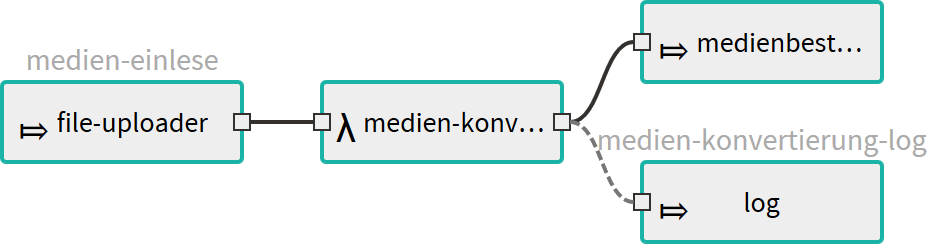
\includegraphics[width=\textwidth]{stream-small.png}

Dies gibt SCDF alle Informationen die es benötigt, um die Konfigurierung vorzunehmen und die Pipeline zu deployen.

SCDF ist extrem leicht erlernbar und ermöglicht mit minimalem Aufwand das Definieren und konfigurieren von Daten-Pipelines.
Es erlaubt außerdem tiefere Konfigurierung des Deployments, wie zum Beispiel das Angeben der Anzahl von Instanzen, die von einem Service erstellt werden sollen, oder das zuweisen von Rechenkapazität für einzelne Services.

\subsection{Spring Cloud Netflix}

Spring Cloud Netflix enthält Unterstützung für die Netflix Open Source Software `Eureka', `Ribbon', `Zuul' und `Hystrix'.
Diese sind dazu gedacht, Anfragen von Clients effizient an die richtigen Microservices weiterzuleiten.

\subsubsection{Eureka}

Eureka verwaltet eine aktuelle Liste von verfügbaren Microservices und gibt auf Anfrage Auskunft über diese.
Die Microservices müssen sich proaktiv bei Eureka registrieren um sichtbar zu sein.

Zusätzlich unterstützt Eureka simplistisches Load Balancing und erlaubt das einführen von komplexerem Load Balancing indem man einen Wrapper dafür schreibt.
Das native Load Balancing verteilt einfach Anfragen in einer festen Reihenfolge an die Services. (Round Robin)

\subsubsection{Ribbon}

Ribbon bietet native Unterstützung für weitere Load Balancing-Verfahren und einfacheres definieren eigener Regeln.
Zusätzlich unterstütz es die Fehlertoleranz des verteilten Systems indem es die Verfügbarkeit von Services prüft und darauf basierend entscheiden kann, wohin Anfragen gerichtet werden sollen.

Ribbon kann direkt mit Eureka zusammenarbeiten um Services zu finden.

\subsubsection{Zuul}

Zuul erfüllt die Aufgaben Anfragen an Microservices entgegenzunehmen, zu filtern, und weiterzuleiten.
Für das Entdecken der Services und Load Balancing ist es in der Lage mit Eureka und Ribbon zusammenzuarbeiten.

Mit Zuul ist es unter Anderem möglich Anfragen zu Authentifizieren, fehlgeschlagene Anfragen zu wiederholen, und Datenverkehr zu Überwachen.
Es ist die zentrale Anlaufstelle für alle Anfragen von Clients und bildet somit den Kern der Anfragenverarbeitung.

\subsubsection{Hystrix}

Hystrix wurde entwickelt um die negativen Auswirkungen von Latenz und Fehlschlägen von Anfragen zwischen Microservices zu vermindern.
Es stoppt das Propagieren von Fehlschlägen, unterbricht zu lange Wartezeiten und erlaubt das Zurückfallen auf Notlösungen.
Dabei muss die Art der Fehlerbehandlung fest vordefiniert werden und kann nicht dynamisch an die aktuelle Performance des Systems angepasst werden.\medskip

Im Zusammenspiel lässt sich mit diesen Projekten der Netflix Open Source Software ein großer Teil des Bedarfs an Infrastruktur für Microservices decken.

\section{Diskussion}

Spring hat es uns ermöglicht, ohne Vorerfahrung innerhalb weniger Tage eine Microservice-Architektur umzusetzen.
Die obigen Beispiele illustrieren deutlich, wie Spring ermöglicht, sich voll und ganz auf die Implementation der Funktionalität der Microservices zu fokussieren.
Der resultierende Code ist sehr einfach wiederzuverwenden und stark abstrahiert.

Die größten Schwierigkeiten einer Microservice-Architektur liegen normalerweise in den Schwierigkeiten verteilter Systeme, wie zum Beispiel der Definition eines Kommunikationsprotokolls.
Die meisten dieser Schwierigkeiten werden von Spring ohne Aufwand seitens der Programmierers gelöst.
Damit bietet Spring eine wichtige Grundlage für gutes Software-Engineering in der Form einer wiederverwendbaren und abstrakten Basis, mit der sich individuell gestaltete Komponenten verbinden lassen.

\bibliographystyle{plain}
\bibliography{bibtex_file}
\end{document}
